\section{Methods}
\label{sec:methods}
Our system follows a modular multi-stage design: an input MRI slice is first segmented to localize the tumor region, the predicted tumor region is cropped and resized, and a classifier predicts one of four classes: glioma, meningioma, pituitary tumor, or no tumor. Finally, Grad-CAM and a summary-generation module are used to provide visual and textual explanations for the prediction.



\subsection{Tumor Localization with ResUNet}
For tumor localization, we use a ResUNet-based~\cite{zhang2018resunet} binary segmentation model. Given an MRI slice $I$, the network predicts a soft tumor mask $\hat{M} \in [0,1]^{H \times W}$, where higher values indicate tumor likelihood. At inference time, a threshold of 0.5 is applied to obtain the final binary mask.

We choose the U-Net~\cite{ronneberger2015unet} family because it is well suited to medical image segmentation with limited annotated data. Its encoder-decoder structure captures semantic context, while skip connections preserve spatial details needed for tumor boundaries. Compared with classification-only CNNs, U-Net directly optimizes pixel-level localization. We also considered more automated or foundation-model-based alternatives such as nnU-Net~\cite{isensee2021nnunet} and SAM-style promptable models~\cite{kirillov2023segment}, but a 2D U-Net-family model offered a better compute-accuracy trade-off for our project timeline.

Our final segmentation model is ResUNet, a residual variant of U-Net. ResUNet keeps the same encoder-decoder and skip-connection structure, but replaces plain convolutional blocks with residual blocks. This improves gradient flow and optimization stability, especially when the network becomes deeper. Since brain tumor regions can vary strongly in size, contrast, and boundary shape, the residual design helps preserve useful low-level and high-level features during mask prediction.

We also evaluated standard U-Net and Attention U-Net as alternatives. Standard U-Net serves as the simplest encoder-decoder baseline, while Attention U-Net tests whether attention gates on skip connections can suppress irrelevant background features. 
Based on the segmentation comparison in Table~\ref{tab:seg-results}, ResUNet performs the best overall, so it is used as the final tumor localization model in the proposed pipeline.
Figure~\ref{fig:segmentation_example} shows an example MRI slice and its corresponding predicted tumor mask produced by the ResUNet segmentation model.


\begin{figure}[!htbp]
    \centering
    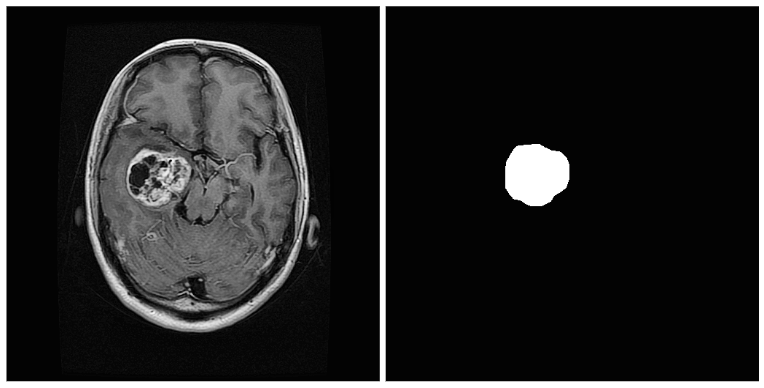
\includegraphics[width=0.5\linewidth]{figures/mri_segmentation_example.png}
    \caption{Left: original brain MRI slice. Right: predicted binary segmentation mask highlighting the tumor region.}
    \label{fig:segmentation_example}
\end{figure}

\subsection{Segmentation Objective}
The segmentation models are trained using a combination of BCE loss and Dice loss. BCE treats segmentation as an independent binary classification problem at each pixel:
\begin{equation}
    \mathcal{L}_{BCE}
    =
    -\frac{1}{N}
    \sum_{i=1}^{N}
    \left[
    M_i \log(\hat{M}_i)
    +
    (1-M_i)\log(1-\hat{M}_i)
    \right],
\end{equation}
where $N$ is the number of pixels, $M_i \in \{0,1\}$ is the ground-truth label for pixel $i$, and $\hat{M}_i \in [0,1]$ is the predicted tumor probability. BCE encourages pixel-wise correctness and provides stable gradients during optimization.

However, tumor segmentation is highly class-imbalanced because the tumor usually occupies only a small portion of the MRI slice. In this setting, a model can achieve low BCE by predicting mostly background. To address this, we also use Dice loss, which directly measures foreground overlap between the predicted mask and the ground-truth mask. The Dice similarity coefficient is defined as:
\begin{equation}
    DSC(\hat{M}, M)
    =
    \frac{2|\hat{M} \cap M| + \epsilon}
    {|\hat{M}| + |M| + \epsilon},
\end{equation}
where $\epsilon$ is a small smoothing constant for numerical stability. Dice loss is then:
\begin{equation}
    \mathcal{L}_{Dice}
    =
    1 - DSC(\hat{M}, M).
\end{equation}
 
The final segmentation objective is:
\begin{equation}
    \mathcal{L}_{seg}
    =
    \lambda \mathcal{L}_{BCE}
    +
    (1-\lambda)\mathcal{L}_{Dice},
\end{equation}
where $\lambda=0.5$ in our experiments. This combined objective balances pixel-level accuracy from BCE with region-level overlap from Dice loss. Such Dice-based objectives are widely used in medical image segmentation because they are more robust to foreground-background imbalance than pixel accuracy alone~\cite{milletari2016vnet,sudre2017generalised}. U-Net-style medical segmentation methods also commonly rely on overlap-based losses or metrics to evaluate tumor-region quality~\cite{ronneberger2015unet}.



\subsection{Segmentation-Guided Classification}
For the segmentation-guided setting, the predicted mask, illustrated in Figure~\ref{fig:segmentation_example}, is converted into a ROI proposal for classification.

We first apply connected-component analysis to the binary mask and select the largest connected component as the predicted tumor region. A bounding box is then fitted around this component and expanded by a 20-pixel margin to preserve nearby anatomical context. The corresponding region is cropped from the original MRI slice and resized to the standard ResNet50 input resolution before classification. If no ROI is available, such as for no-tumor images or empty predicted masks, the full image is resized and used instead. We use this fixed input size because ResNet50 is initialized with ImageNet-pretrained weights, making the fine-tuning setup consistent with the pretrained model while controlling computational cost.

For the final classification setting, we use a dual-input design that combines the segmentation-guided ROI crop with the original full MRI image. The ROI crop provides localized tumor-focused information, while the full image preserves global anatomical context that may be lost during cropping. This design allows the classifier to remain tied to the segmented tumor region while reducing the information loss observed in cropped-only classification.
Figure~\ref{fig:roi_cropping} illustrates this ROI cropping process, where the predicted tumor mask is used to localize the lesion and extract a tumor-centered patch for classification.

\begin{figure}[!htbp]
    \centering
    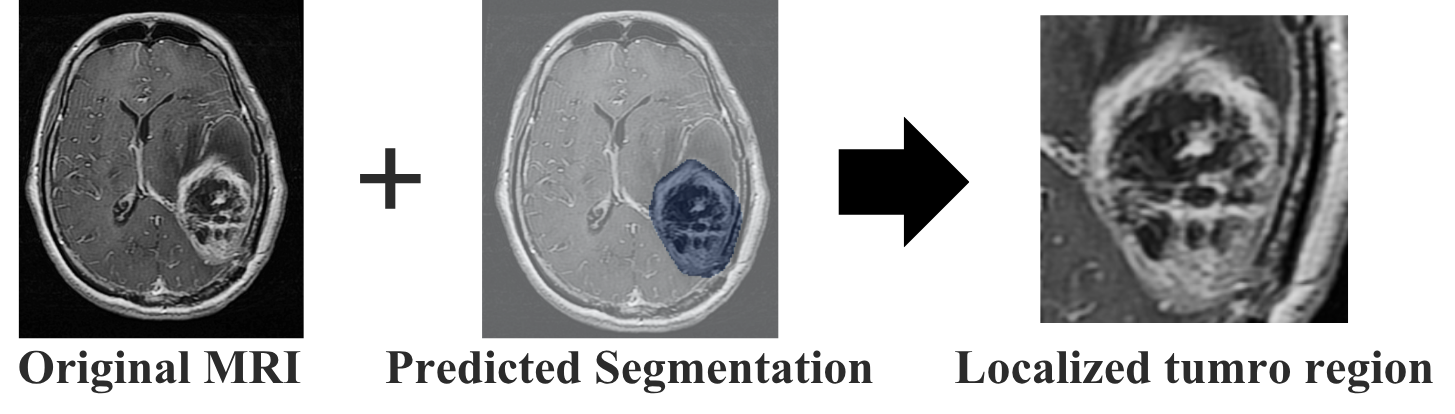
\includegraphics[width=0.97\linewidth]{figures/roi_cropping_example.png}
    \caption{Segmentation-guided ROI cropping for classification.}
    \label{fig:roi_cropping}
\end{figure}

The classifier is based on ResNet50 pretrained on ImageNet~\cite{he2016resnet}. We choose ResNet50 because its residual connections support deep feature learning while reducing vanishing-gradient issues, making it suitable for distinguishing visually similar tumor categories. Compared with larger modern architectures such as Vision Transformers, which typically require larger datasets or more extensive pretraining~\cite{dosovitskiy2021vit}, ResNet50 is a practical transfer-learning backbone for our moderate-sized medical dataset, where fine-tuning pretrained CNNs has been shown to be effective~\cite{tajbakhsh2016convolutional}.

We replace the final fully connected layer with a task-specific four-way classification layer and fine-tune the network using cross-entropy loss. To account for class imbalance, the loss is weighted by inverse class frequency:
\begin{equation}
    \mathcal{L}_{cls}
    =
    - \sum_{c=1}^{C} w_c y_c \log p_c ,
\end{equation}
where $C=4$, $w_c$ is the class weight, $y_c$ is the ground-truth label, and $p_c$ is the predicted probability.




\subsection{Explainability and Summary Generation}
To make the classification decision more interpretable, we use Grad-CAM to identify which image regions contribute most strongly to the ResNet50 prediction. Grad-CAM is applied to the final convolutional block of ResNet50, corresponding to \texttt{layer4} in our implementation. Given a predicted class $c$, Grad-CAM computes the gradient of the class score with respect to the feature maps in this layer. These gradients are then used to weight the feature maps, producing a coarse localization heatmap that highlights the regions most responsible for the prediction. As illustrated in Figure~\ref{fig:gradcam_process}, we normalize this heatmap and overlay it on the input MRI slice, allowing the classifier's attention to be visually compared with the tumor region predicted by the segmentation model.

\begin{figure}[H]
    \centering
    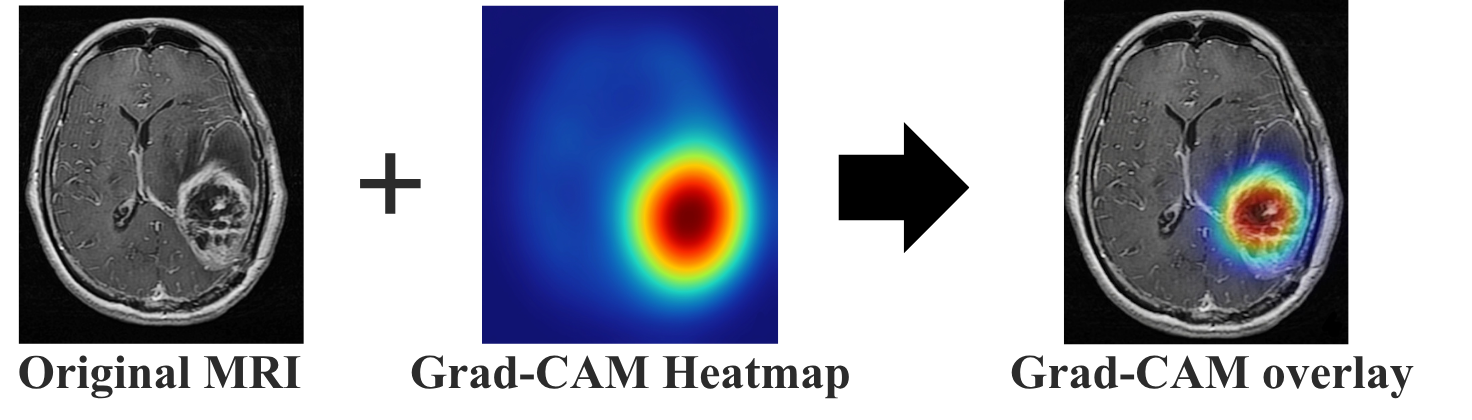
\includegraphics[width=\linewidth]{figures/gradcam_process.png}
    \caption{Grad-CAM visualization process. The heatmap is overlaid on the original MRI slice to highlight regions that contribute most strongly to the classifier prediction.}
    \label{fig:gradcam_process}
\end{figure}

This visual explanation also allows us to check whether the two stages of the pipeline are consistent with each other. To quantify this relationship, we compute a stage-consistency measure between the predicted segmentation mask and the Grad-CAM activation. The segmentation mask is binarized, and the Grad-CAM heatmap is thresholded to identify high-activation regions. We then measure their overlap using IoU. A high overlap suggests that the classifier is focusing on the tumor region proposed by the segmentation model, while a low overlap indicates that the classifier may be relying on background structures or other spurious image cues.

In addition to visual explanations, we generate a structured textual explanation for each prediction. The summary-generation module takes the predicted tumor class, model confidence, Grad-CAM focus region, and optionally the segmentation mask as inputs. It first attempts to produce a summary using a VLM-based generation step conditioned on this model evidence. We use a zero-shot instruction prompt that asks the model to generate three fixed sections: findings, impression, and recommendation. This prompt design is chosen because it does not require task-specific summary examples, while the fixed section format keeps the output clinically structured and easier to validate. If the generated output is unavailable, malformed, or inconsistent with the predicted class, the system falls back to a deterministic class-conditioned template. This hybrid VLM-template design keeps the summary aligned with the classifier output while still allowing more natural clinical language when generation succeeds.

\subsection{Training Strategy}
All models are optimized with Adam and early stopping. The segmentation models are trained using the combined BCE--Dice objective, while the ResNet50 classifier is trained using weighted cross-entropy. Training-time data augmentation is applied online to improve robustness, with random spatial and intensity transformations for segmentation, random rotation, horizontal flipping, and brightness/contrast jittering for classification. Exact hyperparameters are reported in Section~\ref{sec:experiments}.